% UART chapter. Section order is the per-peripheral template enforced by
% python/check_intro_names.py. Vector numbers are frozen by the generator
% (python/generate.py, _mcuMpIrqVectors). Pin lists are generated, not
% written here.
\section{Overview}

The Universal Asynchronous Receiver/Transmitter (\peripheral{UARTx}) is a two-wire, full-duplex asynchronous serial interface with hardware parity. \peripheral{UART0} is the console port used by the boot ROM's Forth interpreter; \peripheral{UART1}, in configurations that include it, is identical.

\begin{itemize}
	\item Independent transmitter and receiver, 8-bit frames, one stop bit
	\item Baud generator from SMCLK with 16 times oversampling (\register{UARTxBR})
	\item Even or odd parity, generated and checked in hardware (\bitfield{UPEN}, \bitfield{PSEL})
	\item Framing, parity and receive-overflow error flags (\bitfield{FEF}, \bitfield{PEF}, \bitfield{OVF})
	\item One-deep transmit queue for back-to-back frames
	\item Three interrupts per port: receive complete, transmit register empty, transmit complete
	\item Latched register reads for stable status during reception
\end{itemize}

\section{Block diagram}

Figure \ref{fig:uart-connection-diagram} shows the two-wire connection to an external device.

\begin{figure}[htpb]
	\centering
	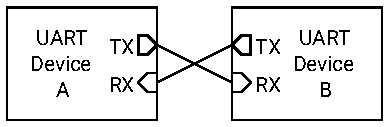
\includegraphics{figures/uart-connection-diagram}
	\caption{UART connection to an external device.}
	\label{fig:uart-connection-diagram}
\end{figure}

\section{Functional description}

\subsection{Frame}

Each wire is unidirectional and idles high. A frame is a start bit (low for one bit time $T_B = 1/\textrm{baud}$), eight data bits LSB first, an optional parity bit, and a stop bit (high for $T_B$). The transmitter may start the next frame immediately after the stop bit or leave the wire idle. Figure \ref{fig:uart-timing-diagram} shows one frame.

\begin{figure}[htpb]
	% Generated by LatexUserGuide.GenerateUartFrameDiagram (make chip).
	\input{include/UartFrameDiagram.tex}
	\caption{One UART frame with the optional parity bit.}
	\label{fig:uart-timing-diagram}
\end{figure}

\subsection{Baud generation}

Both ends must agree on the baud rate, because the receiver has no clock wire and samples each bit at the centre of its expected period. The receiver oversamples at 16 times the baud rate for noise immunity, and the rate is set by the 12-bit \register{UARTxBR}:
\begin{equation*}
\textrm{baud} = \frac{f_\textrm{SMCLK}}{16 \times (\bitfield{BR} + 1)}
\end{equation*}
With SMCLK at 24 MHz, \bitfield{BR} = 12 gives 115,385 baud, \bitfield{BR} = 25 gives 57,692 baud and \bitfield{BR} = 51 gives 28,846 baud, each within 0.2\,\% of the standard rate. The serial engine runs on SMCLK and the register interface on MCLK, so the registers stay readable with SMCLK stopped.

\subsection{Parity}

With \bitfield{UPEN} set the transmitter appends $p = b_7 \oplus \cdots \oplus b_0 \oplus \bitfield{PSEL}$, which is even parity for \bitfield{PSEL} = 0 and odd for 1, and the receiver checks the same function and sets \bitfield{PEF} on a mismatch. Parity detects any odd number of bit errors in a frame and misses any even number.

\subsection{Transmit queue}

A write to \register{UARTxTX} queues one byte. If no frame is in progress the frame starts at once and \bitfield{TEIF} is set immediately; otherwise the byte starts when the current frame ends, and \bitfield{TEIF} is set then. The queue holds one byte, so software waits for \bitfield{TEIF} = 1 or \bitfield{TXBF} = 0 before each write. \bitfield{TCIF} is set when the last stop bit has been sent and the transmitter is idle.

\subsection{Reception and status}

\bitfield{RXBF} is 1 while a frame is being received. When the stop bit has been sampled, the byte is placed in \register{UARTxRX}, \bitfield{RCIF} is set, and \bitfield{FEF}, \bitfield{PEF} and \bitfield{OVF} are updated: \bitfield{FEF} when the stop bit was not high, which usually means the two ends disagree on rate or format; \bitfield{PEF} on a parity mismatch; \bitfield{OVF} when the previous byte had not been read, in which case it is lost. A byte received with \bitfield{FEF} or \bitfield{PEF} set is corrupt. Reading \register{UARTxRX} clears \bitfield{RCIF}, \bitfield{FEF}, \bitfield{PEF} and \bitfield{OVF}; \register{UARTxSR} and \register{UARTxRX} are latched on the falling edge of the memory enable signal, so a read during reception returns one stable sample.

\section{Interrupts and events}

The three interrupt flags in \register{UARTxSR} have enables in \register{UARTxCR} (\bitfield{CIE}, \bitfield{TEIE}, \bitfield{TCIE}); each interrupt is a level asserted while both are set. Table \ref{t:uart-irq} lists the vectors.

\begin{table}[htb]
	\centering
	\caption{\peripheral{UARTx} interrupt vectors.}
	\label{t:uart-irq}
	\begin{tabular}{ l l p{3.8cm} l p{4.6cm} }
	\textbf{Vector} & \textbf{Port} & \textbf{Condition} & \textbf{Set by} & \textbf{Cleared by} \\ \hline
	13 & \peripheral{UART0} & Byte received & \bitfield{RCIF} & Reading \register{UARTxRX}, or writing 1 \\
	\rowcolor{tablehighlightcolor}
	14 & \peripheral{UART0} & Transmit register empty & \bitfield{TEIF} & Writing 1 \\
	15 & \peripheral{UART0} & Transmission complete & \bitfield{TCIF} & Writing 1 \\
	\rowcolor{tablehighlightcolor}
	52 & \peripheral{UART1} & Byte received & \bitfield{RCIF} & Reading \register{UARTxRX}, or writing 1 \\
	53 & \peripheral{UART1} & Transmit register empty & \bitfield{TEIF} & Writing 1 \\
	\rowcolor{tablehighlightcolor}
	54 & \peripheral{UART1} & Transmission complete & \bitfield{TCIF} & Writing 1 \\
	\hline
	\end{tabular}
\end{table}

\section{Programming}

\subsection{Initialisation}

\begin{enumerate}
	\item Select the SMCLK source in \register{SYSCLKCR} (Section \ref{ss:clocks}).
	\item Set the \register{PxSEL} bits of the \pin{TXx} and \pin{RXx} pins, and their \register{PxAFS} fields if the port is relocated.
	\item Write \register{UARTxBR}.\bitfield{BR} for the baud rate.
	\item Write \register{UARTxCR}.\bitfield{UPEN} and \register{UARTxCR}.\bitfield{PSEL} for parity.
	\item Set the interrupt enables required in \register{UARTxCR}.
	\item Set \register{UARTxCR}.\bitfield{UEN}; while it is 0 the port is held in reset.
\end{enumerate}

\subsection{Transmitting a byte}

\begin{enumerate}
	\item Wait for \bitfield{TXBF} = 0 or \bitfield{TEIF} = 1.
	\item Write the byte to \register{UARTxTX}.
\end{enumerate}

\subsection{Receiving a byte}

\begin{enumerate}
	\item Wait for \bitfield{RCIF} = 1.
	\item Read \register{UARTxSR} and reject the byte if \bitfield{FEF} or \bitfield{PEF} is set.
	\item Read \register{UARTxRX}; the read clears the flags.
\end{enumerate}

\section{Usage notes}

\paragraph{Select the SMCLK source before the first frame.} With SMCLK on LFXT (32.768 kHz), as the boot ROM may leave it, each frame takes about 10 \si{\milli\second}.

\paragraph{Read the status before the data.} Reading \register{UARTxRX} clears the error flags, so a handler that reads the byte first cannot tell whether it was corrupt.

\paragraph{Serialize whole messages between harts.} The arbiter makes each register access atomic; bytes from two harts interleave on the wire (Section \ref{ss:multicore-sync}).

\paragraph{Clear \bitfield{TEIF} and \bitfield{TCIF} with a 1 before returning.} Both are levels into the interrupt controller.

\paragraph{Leave \peripheral{UART0} to the console during boot.} The boot ROM's Forth interpreter owns \peripheral{UART0} at 115,200 baud until the application starts (Section \ref{s:startup}).
